


\thispagestyle{empty}


%~
%\tikz[remember picture, overlay] \node  at (current page.center){\includegraphics[width=\paperwidth,height=\paperheight]{images/titlebg}};


~
\vskip 1.75in

\begin{center}


\resizebox{.9\linewidth}{!}{\scshape Some Abstract Algebra}


\vskip 3em

% \tikz[scale=1]{
% \draw (0,0) rectangle (2,2);
% \draw (-0.2, -0.2) rectangle (2.2, 2.2);
% \draw (-0.4, -0.4) rectangle (2.4, 2.4);
% \draw (-0.6, -0.6) rectangle (2.6, 2.6);
% }

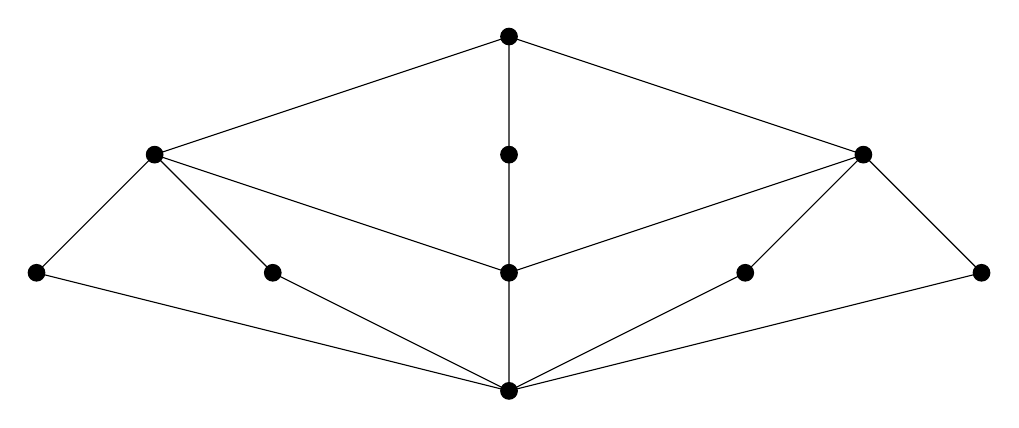
\begin{tikzpicture}[scale=1.5]
	\coordinate (h9) at (0,0);
	\coordinate (h8) at (4,1);
	\coordinate (h7) at (2,1);
	\coordinate (h6) at (0,1);
	\coordinate (h5) at (-2,1);
	\coordinate (h4) at (-4,1);
	\coordinate (h3) at (3,2);
	\coordinate (h2) at (0,2);
	\coordinate (h1) at (-3,2);
	\coordinate (h0) at (0,3);

	\draw[color=black] (h0) -- (h1) -- (h4) -- (h9) -- (h8) -- (h3) -- (h0) -- (h2) -- (h6) -- (h9) -- (h5) -- (h1) -- (h6) -- (h3) -- (h7) -- (h9);
	\foreach \i in {0,...,9}{
	\draw[fill=black, color=black] (h\i) circle (2pt);
	}
\end{tikzpicture}

\vskip 2em

\resizebox{.75\linewidth}{!}{\scshape A Primer and Interactive Workbook}



\vskip 1.5in

\resizebox{.75\linewidth}{!}{\scshape Richard Grassl \quad - \quad Tabitha Mingus}

\vskip .5in

% \resizebox{.2\linewidth}{!}{\scshape 2018}

\end{center}


%\includepdf[pages=-,pagecommand={\thispagestyle{empty}}]{frontmatter/cover2}
%
%

\clearpage






%\addtocontents{toc}{\protect\thispagestyle{plain}}
